\documentclass{cmi}
\usepackage{upgreek}

% Данные поля заполняются редакцией журнала
%\makeatletter
%\newcommand{\@volume}{}
%\newcommand{\@issue}{}
%\newcommand{\@num}{}
%\newcommand{\@pages}{}
\usepackage{subcaption}

\begin{document}

\classify{УДК 123.456, 789.012}

\renewcommand*{\thefootnote}{\fnsymbol{footnote}} %to make a number in end of title delete this line

\title{ШАБЛОН ОФОРМЛЕНИЯ СТАТЬИ В СИСТЕМЕ \LaTeXe{}\\ ДЛЯ~СЕРИИ <<ВЫЧИСЛИТЕЛЬНАЯ МАТЕМАТИКА И~ИНФОРМАТИКА>>%
\footnote{Если статья рекомендована к публикации программным
комитетом научной конференции, это указывается в сноске к названию статьи. Благодарность за финансовую поддержку в подготовке статьи необходимо поместить после заключения.}%
}

\authors{К.А.~Баркалов$^{2,3}$, Е.Н.~Варсеева$^{2}$}

\organizations{$^{1}$Южно-Уральский государственный университет\\
	(454080 Челябинск, пр.~им.~В.И.~Ленина, д.~76),\\ 
	$^{2}$Нижегородский государственный университет им. Н.И. Лобачевского	\\ (603022 Н.~Новгород, просп.~Гагарина, д.~23)\\
	$^{3}$Научно-образовательный математический центр <<Математика технологий будущего>> \\ (603022 Н.~Новгород, просп.~Гагарина, д.~23, корп.~2)
	}

\newcommand{\emailsinsert}{\href{mailto:konstantin.barkalov@itmm.unn.ru}{konstantinbarkalov@itmm.unn.ru}, \href{mailto:kate.varseeva@yandex.ru}{kate.varseeva@yandex.ru}}

% Дата поступления статьи в редакцию
\newcommand{\rdate}{ДД.ММ.ГГГГ}
\emails{\emailsinsert}
\redactiondate{\rdate}

\renewcommand*{\thefootnote}{\arabic{footnote}}
\setcounter{footnote}{0}

% оформление аннотации
\begin{abstract}%
Аннотация должна представлять собой краткое резюме работы, которое должно быть понятным без обращения к самой публикации. Аннотация отражает научное содержание статьи, содержит сведения о решаемой задаче, методах решения, результатах и выводах. Аннотация не должна содержать ссылок на рисунки, формулы, литературу и источники финансирования работы. Объем аннотации~--- от 150 до 250~слов.

\keywords{необходимо указать от 3 до 10 ключевых слов и (или) фраз через запятую.}
\end{abstract}

%Образец цитирования статьи
\forcitation{Баркалов~К.А., Варсеева~Е.Н. Шаблон оформления статей в системе \LaTeXe{} для серии <<Вычислительная математика и информатика>>}

%Верхние колонтитулы
\markboth{К.А.~Баркалов, Е.Н.~Варсеева}{Название статьи с многоточием в случае нехватки горизонтального\ldots}

% Заголовки разделов формируются при помощи команд  \section{}, \subsection{}, \subsubsection{}
\section*{Введение}
\label{sec-intro}

Уфа - важность рассматриваемой задачи химической кинетики с прикладной точки зрения. Обзор разных постановок.

НН - сложность решаемой задачи оптимизации. Обзор методов решения оптимизационных задач, применимых для обратных задач химической кинетики. Необходимость применения параллельных вычислений. 



Структура статьи - кратко

Данный документ содержит примеры правильного оформления статьи в \LaTeXe{}, и
его можно использовать в качестве шаблона. Во введении необходимо описать
проблематику и обосновать актуальность исследования, указать цели и задачи
исследования, а также привести краткое содержание разделов и заключения. В разделе~\ref{sec-feel} представлены требования к содержанию статьи. Раздел~\ref{sec-look} посвящен оформлению статьи. Требования к заключению статьи изложены в разделе~\nameref{sec-conclusion}.


\section{Постановка задачи}
\label{sec-problem}

Уфа

Содержательная постановка задачи. Математическая модель в виде системы ОДУ. Метод решения ОДУ, его свойства. 
Задача идентификации параметров реакции.

\section{Параллельный алгоритм решения задач глобальной оптимизации}
\label{sec-PGSA}
НН
Метод решения оптимизационных задач подобного типа должен учитывать следующую специфику. Во-первых, целевая функция задачи представляет собой «чёрный ящик», поскольку она задаётся не аналитической формулой, а в виде алгоритма, вычисляющего её значения. Во-вторых, даже однократное вычисление значения целевой функции является трудоёмкой операцией, так как требует выполнения численного моделирования.

Указанная специфика исключает возможность применения для решения обратных задач мультистартовых методов, основанных на многократном использовании градиентного спуска. С одной стороны, вычисление градиента в данном случае оказывается чрезмерно дорогостоящим, а с другой — мультистартовые подходы слабо применимы к существенно многоэкстремальным задачам, каковыми и являются обратные задачи химической кинетики.

Перечисленные особенности обратной задачи химической кинетики учитываются в разработанном в Нижегородском университете параллельном алгоритме глобальной оптимизации. Теоретической основой данного алгоритма служит информационно-статистический подход, подробно изложенный в \cite{Strongin2000}. Суть алгоритма заключается в редукции исходной многомерной задачи к эквивалентной одномерной задаче, которая затем решается эффективными методами оптимизации функций одной переменной. Вопросы распараллеливания предложенного алгоритма на различных архитектурах рассматриваются в \cite{Barkalov2016}.

В настоящей статье представлены результаты применения параллельного алгоритма глобального поиска к решению обратной задачи химической кинетики.

\subsection{Задача глобальной оптимизации}

Рассмотрим задачу глобальной оптимизации вида 
\begin{gather}
 \varphi(y^\ast)=\min{\left\{\varphi(y):y\in D\right\}}, \label{problem}\\
 D=\left\{y\in \mathbb{R}^N: a_i\leq y_i \leq b_i, \; a_i,b_i\in \mathbb{R}, \;  1\leq i \leq N\right\} \label{D},
\end{gather}
где целевая функция является <<чёрным ящиком>> и предполагается удовлетворяющей условию Липшица
\[
\left|\varphi(y_1)-\varphi(y_2)\right|\leq L\left\|y_1-y_2\right\|,\; y_1,y_2 \in D,
\]
с константой $L, \; L<\infty,$ неизвестной априори.

Предположение о липшицевости целевой функции типично для многих подходов к построению детерминированных алгоритмов глобальной оптимизации.
Первые методы липшицевой оптимизации были предложены в начале 1970-х годов \cite{Piyavskii1972,Shubert1972}. С тех пор это направление активно развивается \cite{Evtushenko2013,Zilinskas2010,Pinter1996,Jones2009}.

В настоящее время для решения задач с чёрноящичной целевой функцией широко применяются природно-вдохновлённые алгоритмы; см., например, \cite{Yang2013,Gendreau2010,Eiben2015}. Такие алгоритмы так или иначе используют идеи случайного поиска. Благодаря простоте реализации и применения они получили широкое распространение. Однако по качеству (например, по количеству корректно решённых задач из заданного набора) эти алгоритмы уступают детерминированным аналогам \cite{Kvasov2018,Sergeyev2018}.

Одним из эффективных детерминированных методов решения многоэкстремальных задач оптимизации является \textit{информационно-статистический алгоритм глобального поиска} \cite{Strongin2000}. Первоначально предложенный для задач без ограничений, он был успешно обобщён на классы задач с невыпуклыми ограничениями и многокритериальной оптимизации. Для различных версий алгоритма также были предложены методы распараллеливания, учитывающие архитектуру современных вычислительных систем \cite{Barkalov2016,globalizerSystem,Strongin2018}.

Многие современные алгоритмы глобальной оптимизации используют идею понижения размерности при решении многомерных задач; см., например, метод диагональных разбиений \cite{Sergeyev2006} или метод симплексных разбиений \cite{Zilinskas2008}. Параллельный алгоритм глобального поиска, описываемый в данном разделе, использует кривые Пеано \cite{Sergeyev2013,Strongin2000}, непрерывно и однозначно отображающие единичный отрезок $[0,1]$ на $N$-мерный куб $D$ из (\ref{D}). С помощью такого отображения исходная многомерная задача (\ref{problem}) сводится к одномерной задаче
\[
\varphi(y^\ast)=\varphi(y(x^\ast))=\min{\left\{\varphi(y(x)): x\in[0,1]\right\}},
\]
где функция $\varphi(y(x))$ удовлетворяет равномерному условию Гёльдера
\[
\left|\varphi(y(x_1))-\varphi(y(x_2))\right|\leq H\left|x_1-x_2\right|^{1/N}
\]
с константой Гёльдера $H$, связанной с липшицевой константой $L$ соотношением
$ H=2 L \sqrt{N+3}$, а $y(x)$ — кривая Пеано, отображающая $[0,1]$ на $D$.

Отметим, что теоретически кривая Пеано $y(x)$ определяется как предельный объект. Поэтому при практической реализации может быть построена лишь некоторая аппроксимация истинной заполняющей пространство кривой. Некоторые методы построения таких аппроксимаций (называемых \textit{развертками}) рассматриваются в \cite{Sergeyev2013,Strongin2000}. В данном случае точность аппроксимации истинной кривой $y(x)$ зависит от плотности развертки $m$ (которая является параметром ее построения) и имеет порядок $2^{-m}$ по каждой координате.
Примеры разверток при размерности $N=3$ и различных значениях $m$ показаны на рис.~\ref{evolvents}.

\begin{figure}[ht]
\begin{minipage}{0.48\linewidth}
\center{\includegraphics[width=1.0\linewidth]{fig1a.JPG} \\ (a)}
\end{minipage}
\begin{minipage}{0.48\linewidth}
\center{\includegraphics[width=1.0\linewidth]{fig1b.JPG} \\ (b)}
\end{minipage}
\caption{Развертки в трёхмерном пространстве при (a) $m=3$ и (b) $m=4$}
\label{evolvents}
\end{figure}

\subsection{Параллельный алгоритм глобального поиска}

Будем называть процесс вычисления значения функции (включая построение образа $y=y(x)$) \textit{испытанием}, а пару $\{x, z = \varphi(y(x))\}$ -- результатом испытания.
При описании параллельного алгоритма будем использовать термин \textit{итерация} для обозначения одновременного (параллельного) выполнения нескольких испытаний. Число испытаний на $n$-й итерации обозначим $p$, а общее число испытаний, выполненных за все $n$ итераций, обозначим $k(n)$. Иными словами, предполагается, что при выполнении $n$-й итерации имеется в распоряжении $p$ вычислителей (потоков или процессов).

Параллельный алгоритм глобального поиска, используемый в настоящем исследовании (согласно \cite{Strongin2000}), формулируется следующим образом.
Первые $p$ испытаний выполняются в точках $x^0 = 0$, $x^1 = 1$ и в произвольных внутренних точках $x^2, ..., x^{p-1}$ интервала $(0,1)$. Предположим, что завершено $n \geq 1$ итераций метода, в ходе которых проведены испытания в $k=k(n)$ точках $x^i, 0 \leq i \leq k$. Тогда точки $x^{k+1},...,x^{k+p}$ для проведения испытаний на следующей $(n+1)$-й итерации определяются согласно следующим правилам. 

\begin{enumerate}
	\item 
	Перенумеруем прообразы всех точек, в которых уже проведены испытания,  
\begin{equation}\label{y_i}
y^0=y(x^0), y^1=y(x^1),...,y^k=y(x^k)
\end{equation}
по возрастанию их координат, то есть
\begin{equation}\label{x_i}
0=x_0<x_1<\dots <x_k=1,
\end{equation}
и сопоставим им вычисленные значения $z_i=\varphi(y(x_i)), 0\leq i \leq k$.
\item
Вычислим максимальное абсолютное значение первых разделённых разностей
\begin{equation}\label{mu}
\mu = \max_{1 \leq i \leq k}\frac{\left|z_i-z_{i-1}\right|}{\Delta_i},
\end{equation}
где $\Delta_i=\left(x_i-x_{i-1}\right)^{1/N}$. Если $\mu = 0$, полагаем $\mu = 1$.
\item
Для каждого интервала $(x_{i-1}, x_i), \; 1\leq i \leq k,$ вычислим величину
\begin{equation}\label{R}
R(i)=r\mu\Delta_i+\frac{(z_i-z_{i-1})^2}{r\mu\Delta_i}-2(z_i+z_{i-1})
\end{equation}
называемую \textit{характеристикой} интервала; вещественное число $r>1$ является входным параметром алгоритма.

\item 
Упорядочим характеристики $R(i), 1 \leq i \leq k$, по убыванию 
\begin{equation}\label{Rdec}
R(t_1)\geq R(t_2)\geq \dots \geq R(t_{k})
\end{equation}
и выберем $p$ наибольших характеристик с номерами интервалов $t_j, 1\leq j \leq p$.
\item
Проведём новые испытания в точках $x^{k+j}\in(x_{t_j-1},x_{t_j}), 1\leq j\leq p$, вычисляемых по формуле
\[
x^{k+j} = \frac{x_{t_j}+x_{t_j-1}}{2} - \mathrm{sign}(z_{t_j}-z_{t_j-1})\frac{1}{2r}\left[\frac{\left|z_{t_j}-z_{t_j-1}\right|}{\mu}\right]^N.
\]

\end{enumerate}

Алгоритм прекращает свою работу, если хотя бы для одного индекса $t_j, 1 \leq j \leq p,$ выполняется условие $\Delta_{t_j}<\epsilon$; здесь $\epsilon>0$ -- заданная точность. Алгоритм также останавливается, если исчерпано максимально допустимое число испытаний $K_{max}$, установленное до начала вычислений.

%теорема о сходимости алгоритма

Условия сходимости для ПАГП могут быть сформулированы в виде следующей теоремы. Введение описанного выше параллелизма не приводит к возникновению предельных точкек, отличных от предельных точек чисто последовательной схемы, т.е. когда $p = 1$.

\begin{theorem}%
	Пусть $\overline{x}$ есть предельная точка последовательности испытаний $\{x^k\}$, порождаемой ПАГП при минимизации функции $f(x), x\in [0,1],$ удовлетворяющей условию Гельдера с константой $H, 0<H<\infty$; причем число задействованных вычислительных элементов $p, 1<p<\infty$ является фиксированным, а в условии остановки $\epsilon = 0$. Тогда:
	
	\begin{enumerate}
		\item
		сходимость к внутренней точке $\overline{x} \in (0,1) $ является двусторонней;
		\item
		точка $\overline{x}$ локально оптимальна, если функция $f(x)$ имеет конечное число локальных экстремумов;
		\item
		если наряду с $\overline{x}$ существует другая предельная точка $\widehat{x}$, то $f(\overline{x})=f(\widehat{x})$;
		\item
		при любом $k>1$ выполняется неравенство $f(x_k) \geq f(\overline{x})$;
		\item
		если на некотором шаге для величины $r\mu$ из (\ref{R}) выполняется условие $r\mu > 2^{2-1/N}H$;
	\end{enumerate}
	то множество предельных точке последовательности $\{x^k\}$ совпадает с множеством точек глобального минимума $f(x)$.
\end{theorem}
\begin{proof}%
	Доказательство теоремы приведено в работе \cite{Strongin2000}.
\end{proof}


Рассмотрим теоретические свойства параллельного алгоритма, характеризующие его ускорение. Одним из главных показателей эффективности параллельных алгоритмов (в любой области, а не только в глобальной оптимизации) является ускорение по времени
\[
S(p)=T(1)/T(p),
\]
где $T(1)$ -- время, необходимое для решения задачи последовательным алгоритмом, а $T(p)$ -- время решения той же задачи параллельным алгоритмом в системе с $p$ вычислительными элементами. Характеристикой эффективности параллельных алгоритмов (по отношению к алгоритмам оптимизации) также является ускорение по числу итераций
\begin{equation}\label{eq:26}
s(p)=n(1)p/n(p),
\end{equation}
где $n(1)$ -- количество испытаний, выполненных последовательным методом, а $n(p)$ -- количество испытаний, выполненных параллельным методом с $p$ параллельными вычислителями. Эта характеристика особенно важна, поскольку при решении прикладных задач время, необходимое для проведения испытания, превышает время, необходимое для обработки его результатов.

Очевидно, что количество итераций $n(p)$ для последовательного и параллельного алгоритмов глобального поиска будет различаться. Фактически, последовательный АГП при выборе точки $x^{k+1}$ следующей $k+1$ итерации обладает полной информацией, полученной на предыдущих $k$ итерациях. На основе той же информации параллельный алгоритм глобального поиска выбирает $p$ точек $x^{k+j}, 1\leq j \leq p$, а не одну. Это означает, что выбор точки $x^{k+j}$ осуществляется в отсутствии информации о результатах испытаний в точках $x^{k+i}, 1\leq i<j$. Только первая точка $x^{k+1}$ будет совпадать с точкой, выбранной последовательным алгоритмом. Другие точки не будут совпадать с точками, сгенерированными последовательным алгоритмом. Эффективность распараллеливания может снижаться при выполнении таких итераций, поэтому будем называть такие испытания <<избыточными>>, а величина
\[
\lambda(p) = \left\{
   \begin{array}{lr}
     (n(p)-n(1))/n(p), & n(p) > n(1),\\
     0, & n(p)\leq n(1),
   \end{array}
\right.
\]
будет характеризовать избыточность метода.

Рассмотрим последовательности точек испытаний $\left\{x^k\right\}$ и $\left\{y^m\right\}$, сгенерированных соответственно последовательным и параллельным алгоритмами при решении одной и той же задачи со значением $\epsilon = 0$ в условии остановки. Следующая теорема из \cite{Strongin2000} определяет количество вычислительных элементов $p$, которые могут быть задействованы для безызбыточного распараллеливания.

\begin{theorem} Пусть $x^\ast$ -- точка глобального минимума, а $x'$ -- точка локального минимума функции $f(x)$, и выполнены следующие условия:
\begin{enumerate}
	\item
	Выполняется неравенство 
	\begin{equation}\label{eq:28}
	f(x')-f(x^\ast)\leq \delta, \delta>0.
	\end{equation}
	\item
	Начальные $q(l)$ точек испытаний последователного и параллельного алгоритмов совпадают, т.е.
	\[
	\left\{x^1,\dots,x^{q(l)}\right\}=\left\{y^1,\dots,y^{q(l)}\right\},
	\]
	где 
	\[
	\left\{x^1,\dots,x^{q(l)}\right\}\subset\left\{x^k\right\}, \ \left\{y^1,\dots,y^{q(l)}\right\}\subset\left\{y^m\right\}.
	\]
	\item
	Существует точка $y^n\in \left\{y^m\right\}, n<q(l),$ такая, что $x'\leq y^n \leq x^\ast$ or \mbox{$x^\ast \leq y^n \leq x'$}.
	\item
	Для величины $r\mu$ из (\ref{R}) выполняется неравенство
	\[
	r\mu>2^{2-1/N}H,
	\]
	где $H$ -- константа Гельдера целевой функции.
\end{enumerate}

Тогда параллельный алгоритм глобального поиска с использованием двух вычислтельных элементов будет безызбыточным (т.е. $s(2)=2$, $\lambda(2)=0$), если выполняется следующее условие\begin{equation}\label{eq:32}
\left(x_{t_j}-x_{t_j-1}\right)^{1/N} > \frac{4\delta}{M-2^{2-1/N}H}, 1\leq j\leq p,	
\end{equation}
где $t_j$ определяется в соответствии с (\ref{Rdec}).
\end{theorem}

\begin{proof}%
	Доказательство теоремы приведено в работе \cite{Strongin2000}.
\end{proof}

\begin{corollary} Пусть у целевой функции $f(x)$ имеется $Q$ точек локального минимума $\left\{x'_1,\dots,x'_Q\right\}$, для которых выполнено условие (\ref{eq:28}), и пусть существуют точки $y^{n_i}, 1\leq i \leq Q,$ такие, что
\[
y^{n_i}\in \left\{y^1,\dots,y^{q(l)}\right\},
\]
\[
\alpha_i \leq y^{n_i} \leq \alpha_{i+1}, \; \alpha_i, \alpha_{i+1} \in \left\{x^\ast, x'_1,\dots,x'_Q\right\}, \; 1\leq i \leq Q.
\]

Тогда, если условия теоремы выполнены, параллельный алгоритм глобального поиска с $Q+1$ параллельными вычислительными элементами будет безызбыточным (т.е. $s(Q+1)= Q+1$, \mbox{$\lambda(Q+1)=0$}), при  выполнении условия (\ref{eq:32}).

\end{corollary}

Следствие из теоремы играет особую роль в решении многомерных задач, редуцированных к одномерным с помощью разверток типа кривой Пеано $y(x)$. Развертка $y(x)$, являющаяся приближением к кривой Пеано, имеет эффект <<расщепления>> точки глобального минимума $y^\ast\in D$ на несколько прообразов в интервале $[0,1]$. Если функция $\varphi(y)$ имеет единственный глобальный минимум в $D$, то <<редуцированная>> одномерная функция $f(x)$ может иметь до $2^N$ локальных экстремумов, близких (по значению) к глобальному (см. \cite{Strongin2000}). Применяя параллельный АГП для минимизации подобной функции, можно достичь безызбыточности распараллеливания при использовании до $2^N+1$ вычислительных элементов.

%Russian
Рассматриваемый вариант распараллеливания является \textit{синхронным}, когда переход к следующей итерации осуществляется только после полного завершения текущей, то есть после окончания последнего испытания текущей итерации. 

Конкретная реализация этой схемы распараллеливания будет зависеть от архитектуры компьютерной системы, а также от требований к программному обеспечению, необходимому для вычисления значений целевой функции. В настоящем исследовании для проведения испытаний требовалось решить систему ОДУ (для решения этой задачи использовался модифицированный методы Рунге-Кутты 4-го порядка). Распараллеливание было организовано с использованием общей памяти и схемы мастер-рабочие. Алгоритм глобального поиска был запущен в потоке-мастере, остальные (подчиненные) потоки проводили параллельные испытания в рамках шага 5 алгоритма. При этом время проведения одного испытания составляло порядка 0.1 секунды, таким образом, накладные расходы на синхронизацию между потоками не оказывали существенного влияния на эффективность распараллеливания.


%Локальное уточнение

После определения с помощью АГП точки, являющейся оценкой глобального минимума, из нее запускается локальный метод. Мы использовали метод Хука--Дживса, который относится к классу методов нулевого порядка. Его правила вычисления представляют собой комбинацию исследовательского поиска (для выбора направления) и последующего поиска в выбранном направлении \cite{Himmelblau75}.

Исследующий поиск определяется следующим образом: 
\begin{itemize} 
  \item Вначале определяется величина шага: она является различной для каждого координатного направления и может изменяться во время поиска. 
  \item Шаг поиска считается успешным, если значение целевой функции в новой точке не превышает значение целевой функции в исходной точке. 
  \item Если шаг является неуспешным, то нужно вернуться к исходной точке и сделать шаг в обратном направлении. 
  \item После перебора всех $N$ координатных направлений исследовательский поиск завершается; полученная точка является базовой точкой для поиска по образцу.
\end{itemize}

Поиск по образцу состоит из выполнения одного шага от полученной базовой точки вдоль линии, соединяющей ее с предыдущей базовой точкой.

Рис. \ref{fig:fig1} иллюстрирует работу локального алгоритма. Показаны линии уровня целевой функции; темные точки соответствуют успешным, а светлые -- неуспешным шагам, проведенным в ходе исследовательского поиска.

\begin{figure} 
	\begin{center} 
			
\includegraphics[width=0.8\linewidth]{pic/fig1.pdf} 
			\caption{Иллюстрация работы метода Хука-Дживса} %%  подпись к рисунку 
			\label{fig:fig1} 
	\end{center} 
\end{figure}	



\section{Результаты численных экспериментов}
\label{sec-result}

Вычислительные эксперименты проводились на узле суперкомпьютера <<Лобачевский>> в следующей конфигурации: операционная система Linux CentOS 8.2, 2 процессора Intel Xeon Platinum 8558 2.1/4GHz (48 ядер каждый), оперативная память 2048 ГБ. 
Все рассмотренные алгоритмы реализованы на С++, использовался компилятор Intel С++ Сompiler 2023 с поддержкой OpenMP.

Выбор оптимальных кинетических параметров осуществлялся следующим образом. Были получены экспериментальные данные для 18 различных температур проведения реакции. Далее, для каждой из этих температур решалась обратная задача и выбирались константы скоростей реакций, минимизирующие функцию (6) отклонения расчётных концентраций от экспериментальных для каждой температуры. Далее предэкспоненциальный множитель и энергии активации, входящие в уравнения линейно, искались с помощью метода наименьших квадратов.


Таким образом, с помощью параллельного АГП было решено 18 обратных задач, каждая для своей температуры.
Параллельный алгоритм запускался со следующими параметрами: плотность построения развертки $m=10$, параметр надежности $r=1.5$, точность глобального поиска $\epsilon = 10^{-2}$, локального уточнения $\delta = 10^{-4}$; максимальное число итераций глобального поиска $K_{max} = 64 000$, локального поиска $K_{max} = 500$. Число потоков варьировалось от 1 до 128.
В таблице \ref{tab:scalability} приведены усредненные (по всем 18 задачам) оценки времени работы и ускорения параллельного алгоритма.  

%Критерий остановки - по числу испытаний, максимальное число испытаний 64 000 для каждой температуры (в сумме 64 000 * 18 = 1 152 000 испытаний за полный эксперимент)
%Число потоков: от 1 до 128.
%r = 1.001
%После работы АГП запускался локальный метод.

\begin{table}[h]
\noindent
\caption{Зависимость времени решения и ускорения от числа потоков}
\label{tab:scalability}
\centering
\begin{tabular}{|c|c|c|}
\hline
\textbf{P} & \textbf{Время решения, с} & \textbf{Ускорение} \\
\hline
1   & 1170,00  & --- \\
2   & 600,27  & 1,95 \\
4   & 308,34  & 3,79 \\
8   & 162,82  & 7,19 \\
16  & 87,95   & 13,30 \\
32  & 54,43   & 21,50 \\
64  & 47,90   & 24,42 \\
128 & 51,64   & 22,65 \\
\hline
\end{tabular}
\end{table}

С помощью алгоритма глобального поиска для каждой температуры были получены наборы констант скоростей, минимизирующие функцию отклонения расчётных концентраций от экспериментальных (6) для каждой температуры. Довески из формулы (6) были подобраны экспериментально: \{1., 1., 1., 1., 1., 4.4\}.

После того, как с помощью параллельного АГП были получены наборы констант скоростей для каждой температуры, осуществлялся поиск предэкспоненциального множителя $k_0$ и энергии активации $E_a$ (Дж/моль). Для этого метод наименьших квадратов применялся к соотношению, полученному логарифмированием уравнения Аррениуса:
\begin{equation}
ln k=ln k_0 - \frac{E_a}{RT},
\end{equation}
где R - универсальная газовая постоянная, Дж/(моль $\cdot$ K); T - температура, K.

Здесь в качестве k подставляются полученные параллельным алгоритмом глобального поиска значения констант скоростей, соответствующие различным температурам T.

Далее методом наименьших квадратов были рассчитаны значения для k0 и Ea для всех стадий. Полученные значения приведены в таблице 2.

\begin{table}[h]
\noindent
\caption{Рассчитанные кинетические параметры реакций (1)}
\label{tab:scalability}
\centering
\begin{tabular}{|c|c|c|}
\hline
\textbf{№ реакции} & \textbf{lnk$_0$} & \textbf{E$_a$, кДж/моль} \\
\hline
1   & 15,09  & 73,28 \\
2   & 4,65  & 7,51 \\
3   & 3,19  & 8,88 \\
4   & 4,28  & 5,87 \\
4'  & 10,6   & 57,31 \\
\hline
\end{tabular}
\end{table}

Далее расчётные концентрации были пересчитаны с учётом k$_0$ и E$_a$, полученных методом наименьших квадратов. Полученные расчётные концентрации для разных температур были сопоставлены с экспериментальными концентрациями.

На рисунке 2 представлены графики зависимости экспериментальных и расчётных концентраций от температуры для C$_3$H$_8$, H$_2$O, CO$_2$, H$_2$, CH$_4$, C$_2$H$_6$. Экспериментальные данные обозначены синим цветом, а расчётные - оранжевым. Показано, что модель соответствует эксперименту и может использоваться для прогнозирования состава продуктов паровой конверсии углеводородов.

\begin{figure}[ht]
    \centering
    \begin{subfigure}[b]{0.45\linewidth}
        \centering
        \includegraphics[width=\linewidth]{C3H8.jpg}
        \caption{C$_3$H$_8$}
    \end{subfigure}
    \hfill
    \begin{subfigure}[b]{0.45\linewidth}
        \centering
        \includegraphics[width=\linewidth]{H2O.jpg}
        \caption{H$_2$O}
    \end{subfigure}

    \begin{subfigure}[b]{0.45\linewidth}
        \centering
        \includegraphics[width=\linewidth]{CO2.jpg}
        \caption{CO$_2$}
    \end{subfigure}
    \hfill
    \begin{subfigure}[b]{0.45\linewidth}
        \centering
        \includegraphics[width=\linewidth]{H2.jpg}
        \caption{H$_2$}
    \end{subfigure}

    \begin{subfigure}[b]{0.45\linewidth}
        \centering
        \includegraphics[width=\linewidth]{CH4.jpg}
        \caption{CH$_4$}
    \end{subfigure}
    \hfill
    \begin{subfigure}[b]{0.45\linewidth}
        \centering
        \includegraphics[width=\linewidth]{C2H6.jpg}
        \caption{C$_2$H$_6$}
    \end{subfigure}
    \caption{Сопоставление экспериментальных и расчётных концентраций}
\end{figure}

Уфа - содержательная интерпретация полученных результатов.

\section*{Заключение}
\label{sec-conclusion}



В планы дальнейших работ входит также использование других схем распараллеливания, способных повысить эффективность использования параллельных вычислительных систем для решения задач глобальной оптимизации. Сложности с достижением значительных показателей ускорения объясняются следующими двумя обстоятельствами. 

Во-первых, при реализации параллельного алгоритма была применена синхронная схема распараллеливания. Управляющий поток-мастер (в котором работал метод оптимизации) при выполнении  шага 5 алгоритма ожидал окончания проведения всех испытаний, проводимых рабочими потоками. В решаемой задаче время проведения одного испытания зависит от времени решения системы ОДУ и может варьироваться в зависимости от конкретных значений параметров. Возможный путь к повышению эффективности распараллеливания --- реализация асинхронной схемы проведения испытаний на шаге 5 алгоритма. В этом случае результаты испытания, полученные одним из вычислителей, могут быть отправлены для обработки мастеру немедленно, без ожидания окончания других испытаний. После чего вычислитель получает от мастера новую точку, в которой начнет проведение очередного испытания. Асинхронная схема распараллеливания, теоретически, способна обеспечить полную загрузку задействованных вычислительных ресурсов даже в том случае, когда время выполнения испытаний различно в разных точках области поиска.
 
Во-вторых, при масштабном распараллеливании <<узким местом>> становится локальный поиск, который выполняется для уточнения решения после завершения фазы глобального поиска. Локальный поиск требует незначительного (по сравнению с глобальным) числа поисковых испытаний, но эти испытания выполняются последовательно. И при параллельном запуске это незначительное число последовательных испытаний становится сопоставимым с числом параллельных итераций глобального поиска. В дальнейшем планируется использовать параллельную реализацию метода локального поиска на завершающем этапе работы, что способно повысить эффективность распараллеливания в целом.

Наконец, планируется развитие математических основ используемых алгоритмов параллельной глобальной оптимизации. 
В задаче поиска параметров модели, обеспечивающих минимум невязки между расчетными и экспериментальными данными, теоретическое значение целевой функции в точке глобального минимума является известным --- оно равно нулю.
При этом точка глобального минимума (соответствующая лучшим значениям параметров модели) является неизвестной и подлежит определению.
На практике нулевое значение невязки может и не достигаться, если исследуемая модель плохо соответствует эксперименту, но в таком случае целевая функция будет положительной.  
Информацию о нижней границе значений целевой функции можно использовать для разработки нового алгоритма оптимизации, который позволит как гарантировать сходимость к глобальному минимуму, так и ускорить процесс его отыскания.


\vspace{1em}
{\it Работа выполнена при финансовой поддержке Министерства образования и науки Российской Федерации, проект № FSWR-2026-0007.}






\section{Содержание статьи}
\label{sec-feel}

Редакция принимает не публиковавшиеся ранее научные работы следующих трех
видов: обзорная статья (объемом не более 20 страниц формата A4), полная статья
(объемом не более 14 страниц формата A4), краткое сообщение (объемом от 4 до 6
страниц формата A4). Статьи объемом более 20 страниц формата A4 могут быть
приняты к печати только после предварительного согласования с редакцией.
В объем статьи \emph{не включается} перевод названия, списка авторов,
аннотации, списка литературы и проч. на английский язык.

\emph{Обзорная статья} содержит анализ, сопоставление и выявление наиболее
важных и перспективных направлений развития определенного направления науки в
соответствии с тематикой журнала. Обзорная статья должна носить проблемный
характер, демонстрировать различные взгляды на развитие научных знаний,
содержать выводы, обобщения и сводные данные.

\emph{Научная статья} отражает результаты завершенного научного исследования и
имеет обычно следующую логическую структуру.
\begin{itemize}
	\item[--]Введение~--- проблематика, цели и задачи исследования.

	\item[--]Обзор работ по теме исследования (может включаться во
	введение).

	\item[--]Теоретическая часть~--- формализованная постановка задачи,
	описание и аналитическое исследование предлагаемых авторами подходов,
	методов и алгоритмов.

	\item[--]Реализационная часть~--- описание программной реализации
	предложенных подходов, методов и алгоритмов.

	\item[--]Экспериментальная часть~--- результаты вычислительных
	экспериментов, подтверждающих адекватность и эффективность предложенных
	моделей, методов и алгоритмов; сравнение описанного подхода с ранее
	известными.

	\item[--]Заключение~--- краткая сводка результатов, полученных в работе, итоговые выводы и направления дальнейших исследований.
\end{itemize}

\section{Оформление статьи}
\label{sec-look}

\subsection{Параметры страницы и основного текста}

Страница статьи должна размеры $297\times210$~мм (формат А4). Все поля страницы должны
иметь одинаковый размер~--- 25~мм.

Не допускается использование нумерации, принудительных разрывов страниц и
колонтитулов.

В тексте статьи используется шрифт Computer Modern. Абзац оформляется шрифтом
размером 11~пт с выравниванием по ширине страницы, одинарным интервалом между
строками и автоматической расстановкой переносов. Абзацы не разделяются
интервалами и начинаются с красной строки с отступом 7~мм.

\vspace{1em}
\fbox{
\begin{minipage}{\dimexpr\linewidth-2cm\relax}
	Правильные параметры страницы и основного текста уже настроены в
	стилевом файле \texttt{cmi.cls}, поэтому специальных усилий для их
	соблюдения предпринимать не требуется.
	
	Не следует самостоятельно вносить правки в стилевой файл. 
	Вопросы и предложения по содержанию стилевого файла следует направлять техническому редактору журнала.
\end{minipage}
}
\hfill
\begin{minipage}{0.5cm}
	\resizebox{!}{1cm}{!}
\end{minipage}

\subsection{Заголовки}

Заголовки допускаются трех уровней и помещаются в текст с помощью команд
\verb=\section{Название}=, \verb=\subsection{Название}= и
\verb=\subsubsection{Название}=. Для оформления заголовков без нумерации
используются соответствующие команды со звездочкой, например,
\verb=\section*{Введение}=.

Завершающая точка в названии заголовка не ставится. В названии заголовка раздела не должно быть переносов. В случае многострочного заголовка завершающие строку предлоги и союзы следует переносить на следующую строку.

\subsection{Определения, формулы, утверждения, леммы и теоремы}

Определения, формулы, утверждения, леммы и теоремы оформляются в виде отдельного абзаца и нумеруются в соответствии с порядком их появления в тексте статьи, начиная с единицы.  Далее приведены примеры исходного кода и полученного оформления. Для
построения теоремы без номера используйте окружение \verb=theorem*=.
Расшифровка обозначений, принятых в формуле, производится в порядке их использования в формуле.

\vspace{1em}
\noindent
\begin{minipage}[t]{0.48\linewidth}
\begin{Verbatim}[frame=single]
\begin{theorem}%
    Для любого натурального числа
    $n > 2$ уравнение $a^n + b^n =
    c^n$ не имеет натуральных
    решений $a$, $b$ и $c$.
\end{theorem}
\begin{proof}%
    Оставляется читателю
    в качестве упражнения.
\end{proof}
\end{Verbatim}
\end{minipage}
\hfill
\begin{minipage}[t]{0.48\linewidth}
	\begin{theorem}%
		Для любого натурального числа
		$n > 2$ уравнение $a^n + b^n =
		c^n$ не имеет натуральных
		решений $a$, $b$ и $c$.
	\end{theorem}
	\begin{proof}%
		Оставляется читателю
		в качестве упражнения.
	\end{proof}
\end{minipage}
\vspace{1em}

\vspace{1em}
\noindent
\begin{minipage}[t]{0.48\linewidth}
\begin{Verbatim}[frame=single]
\begin{lemma}%
    Производная дифференцируемой
    функции в точке локального
    экстремума равна нулю.
\end{lemma}
\end{Verbatim}
\end{minipage}
\hfill
\begin{minipage}[t]{0.48\linewidth}
	\begin{lemma}%
		Производная дифференцируемой
		функции в точке локального экстремума
		равна нулю.
	\end{lemma}
\end{minipage}
\vspace{1em}

\vspace{1em}
\noindent
\begin{minipage}[t]{0.48\linewidth}
\begin{Verbatim}[frame=single]
\begin{proposition}%
    Если $n$~--- натуральное число,
    то число $n^2 - n$ является
    четным.
\end{proposition}
\end{Verbatim}
\end{minipage}
\hfill
\begin{minipage}[t]{0.48\linewidth}
	\begin{proposition}%
		Если $n$~--- натуральное число,
		то число $n^2 - n$ является
		четным.
	\end{proposition}
\end{minipage}
\vspace{1em}

\vspace{1em}
\noindent
\begin{minipage}[t]{0.48\linewidth}
\begin{Verbatim}[frame=single]
\begin{corollary}%
    Для любого целого числа $n$,
    которое не делится на 2 и на 5,
    можно подобрать число, состоящее
    только из девяток, которое
    делится на $n$.
\end{corollary}
\end{Verbatim}
\end{minipage}
\hfill
\begin{minipage}[t]{0.48\linewidth}
	\begin{corollary}%
		Для любого целого числа $n$,
		которое не делится на 2 и на 5,
		можно подобрать число, состоящее
		только из девяток, которое
		делится на $n$.
	\end{corollary}
\end{minipage}
\vspace{1em}

\vspace{1em}
\noindent
\begin{minipage}[t]{0.48\linewidth}
\begin{Verbatim}[frame=single]
\begin{definition}%
    Реляционное отношение находится
    в \emph{третьей нормальной
    форме} тогда и только тогда,
    когда оно находится во второй
    нормальной форме, и отсутствуют
    транзитивные функциональные
    зависимости неключевых атрибутов
    от ключевых.
\end{definition}
\end{Verbatim}
\end{minipage}
\hfill
\begin{minipage}[t]{0.48\linewidth}
	\begin{definition}%
		Реляционное отношение находится
		в \emph{третьей нормальной
		форме} тогда и только тогда,
		когда оно находится во второй
		нормальной форме, и отсутствуют
		транзитивные функциональные
		зависимости неключевых атрибутов
		от ключевых.
	\end{definition}
\end{minipage}
\vspace{1em}

\vspace{1em}
\noindent
\begin{minipage}[t]{0.48\linewidth}
\begin{Verbatim}[frame=single]
\begin{remark}%
    Производная дифференцируемой
    функции в точке локального
    экстремума равна нулю.
\end{remark}
\end{Verbatim}
\end{minipage}
\hfill
\begin{minipage}[t]{0.48\linewidth}
	\begin{remark}%
		Производная дифференцируемой
		функции в точке локального
		экстремума равна нулю.
	\end{remark}
\end{minipage}
\vspace{1em}

\vspace{1em}
\noindent
\begin{minipage}[t]{0.48\linewidth}
\begin{Verbatim}[frame=single]
\begin{example}%
    Функция $f(x) = x^{2k}$,
    где $x \in R$ и $k in Z$,
    является четной.

    Функция квадратичной волны
    определяется следующим образом:
    \begin{equation}
        f^I(x,y) =
        \begin{cases}
            0, & \mbox{если }
            d(x,y) > \varepsilon\\
            1, &
            \mbox{в противном случае},
        \end{cases}
    \end{equation}
    где $\varepsilon$~--- наперед
    заданный критерий останова
    вычислений.
\end{example}
\end{Verbatim}
\end{minipage}
\hfill
\begin{minipage}[t]{0.48\linewidth}
	\begin{example}%
		Функция $f(x) = x^{2k}$,
		где $x \in R$ и $k \in Z$,
		является четной.

		Функция квадратичной волны
		определяется следующим образом:
		\begin{equation}
			f^I(x,y) =
			\begin{cases}
				0, &\mbox{если }
				d(x,y) > \varepsilon\\
				1, &
				\mbox{в противном случае},
			\end{cases}
		\end{equation}
		где $\varepsilon > 0$~--- наперед
		заданный критерий останова
		вычислений.
	\end{example}
\end{minipage}
\vspace{1em}

\subsection{Рисунки}

Подпись рисунка начинается с ключевого слова <<Рис. {<номер рисунка>}.>>, выделенного полужирным шрифтом, за которым следует название рисунка обычным шрифтом.  Подпись рисунка выравнивается по центру и помещается под рисунком. Нумерация рисунков сквозная. В конце подписи рисунка точка не ставится, как показано на рис.~\ref{myfigure}.  В случае многострочного названия рисунка завершающие строку предлоги и союзы следует переносить на следующую строку. 

Необходимо использовать черно-белые рисунки или рисунки в градациях серого цвета (если это не приводит к потере информативности) с разрешением не менее 300~dpi. Рисунки желательно располагать в непосредственной близости от первой ссылки на них.

При значительном количестве рисунков рекомендуется группировать их с помощью окружения \verb|minipage| в одном окружении \verb|figure|, как это сделано на рис.~\ref{fig:Scalability}.

Подпись к единственному в статье рисунку не оформляется и в перекрестных ссылках на него не используется номер.

\begin{figure}[h]%
	\centering%
	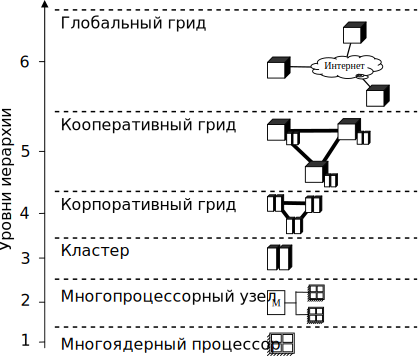
\includegraphics[scale=0.8]{myfigure}%
	\caption{Структура многопроцессорной иерархии}%
	\label{myfigure}%
\end{figure}%

\begin{figure}[!ht]
	\begin{minipage}[t]{1.0\textwidth}
		\centering
		\includegraphics[width=0.495\linewidth]{pic/pic-speedup-gpu-rw-100K.eps}
		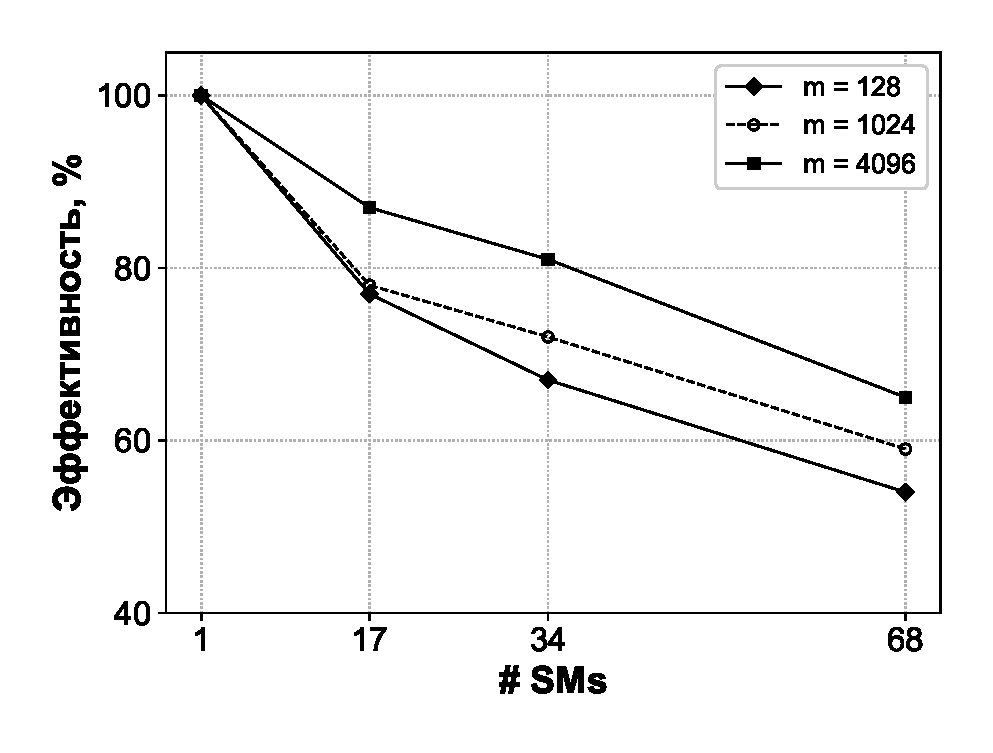
\includegraphics[width=0.495\linewidth]{pic/pic-efficiency-gpu-rw-100K.eps}
		\\а) синтетический ряд Random Walk ($n=10^5$)
	\end{minipage}
	
	\begin{minipage}[t]{1.0\textwidth}
		\centering
		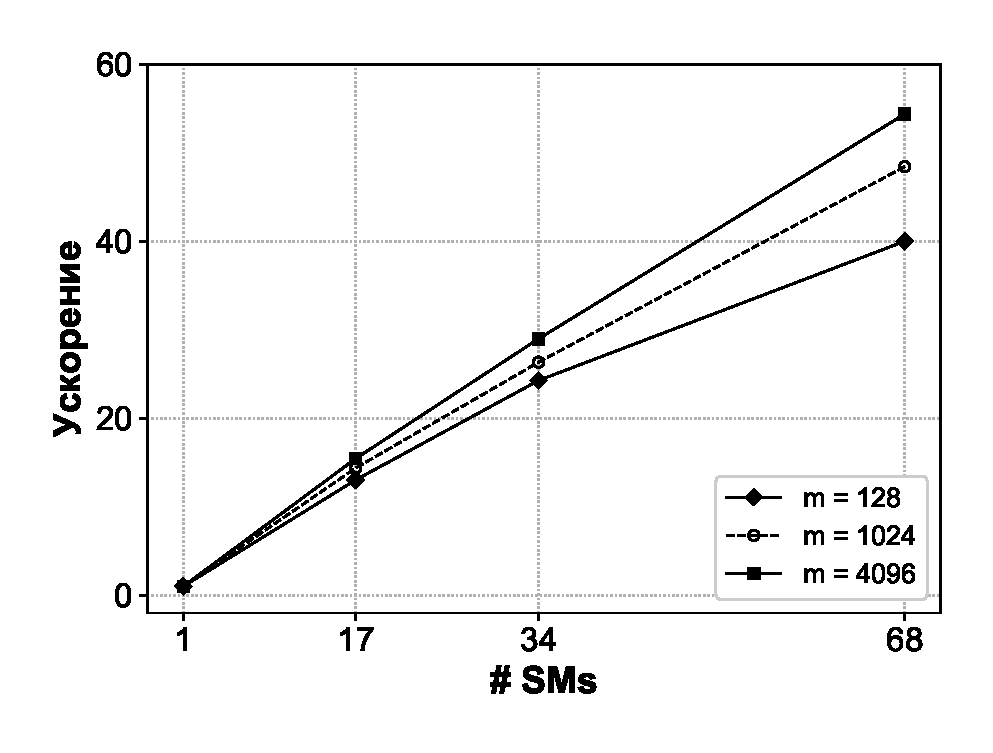
\includegraphics[width=0.495\linewidth]{pic/pic-speedup-gpu-ecg-100K.eps}
		\includegraphics[width=0.495\linewidth]{pic/pic-efficiency-gpu-ecg-100K.eps}
		\\б) реальный ряд ЭКГ ($n=10^5$)
	\end{minipage}
	\caption{Ускорение и параллельная эффективность алгоритма}
	\label{fig:Scalability}
\end{figure}

\subsection{Таблицы}

Каждая таблица должна быть выровнена по центру и иметь подпись, которая начинается с ключевого слова <<Таблица {<номер таблицы>}.>>, выделенного полужирным шрифтом, и помещается над таблицей с выравниванием по левому краю таблицы. В этой же строке помещается название таблицы обычным шрифтом. Нумерация таблиц сквозная. Завершающая точка в названии таблицы не ставится.

Таблицы желательно располагать в непосредственной близости от первой ссылки на них. Недопустимо разрывать между страницами строки таблицы. Нежелательно располагать несколько таблиц подряд, не перемежая их текстом. 

\begin{table}[h]%
	\centering
	\ttabbox[\FBwidth]{	\caption{Аппаратная платформа экспериментов}\label{tab1}}
	{\begin{tabular}{|l|l|}
			\hline
			\multicolumn{1}{|c|}{\bf Характеристика} &
			\multicolumn{1}{|c|}{\bf Значение} \\
			\hline
			Число выч. узлов/процессоров/ядер &
			736/1472/8832 \\
			\hline
			Тип процессора &
			Intel Xeon X5680 (Gulftown, 6~ядер по 3.33~ГГц) \\
			\hline
			Оперативная память &
			3~Тб (DDR3-1333) \\
			\hline
			Дисковая память &
			64~Тб, твердотельные накопители Intel \\
			\hline
			Тип системной сети &
			3D~тор (60~Гбит/с, макс. задержка 1~$\upmu$s) \\
			\hline
			Тип управляющей сети &
			InfiniBand QDR (40~Гбит/с, макс. задержка 2~$\upmu$s) \\
			\hline
			Сервисные сети &
			Сервисная сеть СКИФ ServNet v.4 \\
			& Сеть глобальной синхронизации \\
			\hline
			Пиковая производительность & 117~Тфлопс \\
			\hline
			Производительность на тесте & 100.4~Тфлопс \\
			LINPACK & \\
			\hline
	\end{tabular}}
\end{table}

\subsection{Исходные тексты (псевдокод) алгоритмов}

Исходные тексты программ оформляются в виде рисунков с помощью команды \verb=\code=. Например, \verb|\code[10.5cm]{frame=single}{mycode.txt}{Алгоритм сортировки...}| вставит рисунок, подобный рис.~\ref{mycode.txt}. Обязательно использование <<лесенки>> для отражения вложенности языковых конструкций.

\code[10.5cm]{frame=single}{mycode.txt}{Алгоритм сортировки массива по возрастанию выбором}

\subsection{Перекрестные ссылки на рисунки, таблицы, разделы и формулы}

В перекрестных ссылках на таблицы и рисунки используются сокращения постоянной части их подписи, начинающиеся со строчной буквы, и номер. Например: рис.~\ref{myfigure} и рис.~\ref{fig:Scalability}, табл.~\ref{tab1}. Перекрестные ссылки на рисунки, таблицы, разделы и формулы вставляются с помощью команды \verb=\ref{метка}=.

\subsection{Прочие правила оформления текста}

При написании вещественных чисел для разделения целой и дробной частей должна использоваться точка.

В основном тексте используются <<такие>> кавычки (вместо ``таких'' и др.). <<Такие>> кавычки обозначаются в коде статьи \verb=<<таким>> образом=.

\emph{Вместо буквы <<ё>>} необходимо использовать <<е>>, за исключением имен собственных и особых случаев.

\emph{Дефис} (в коде статьи обозначается минусом \verb=-=) ставится в составных словах, в остальных случаях используется тире (тройной минус \verb=---=). Например: <<супруги Жолио-Кюри>> (двойная фамилия), <<нормальная форма Бойса---Кодда>> (две фамилии).

\emph{Тире} отделяется от предшествующего текста неразрывным пробелом: \verb*'Знание~--- сила'.

\emph{Неразрывный пробел}~\verb'~' ставится между очень короткой формулой и связанным с ней по смыслу словом: \verb'число~$N$ в~$k$~раз' \verb'больше, чем~$n$'.

\emph{Сокращения} из нескольких слов разделяются неразрывными пробелами (\verb=~=), за исключением общеупотребительных, например: «745~мм~рт.~ст.», «т.е.».

Для написания дат используется формат ДД.ММ.ГГГГ, например: 05.05.2012, 03.02.1971.

Единицы измерения указываются в русскоязычном варианте (при наличии такового) и отделяются от числа неразрывным пробелом. Например: 3.2~ГГц, 5~Тб, 30~м/с$^2$, 70~Дж/моль, 20~$^\circ$C, 50~\%.

Если после текста статьи остается свободным пространство объемом более четверти листа, следует поместить переводную часть на этой же странице, отделив ее горизонтальной чертой.
Если переводная часть статьи начинается с новой страницы, горизонтальная черта перед переводом названия статьи не ставится.


\subsection{Перевод названия, аннотации, ключевых слов и списка литературы}

В переводе названия статьи на английский язык используются только прописные буквы, переносы в названии недопустимы.

В переводе названия, аннотации и ключевых слов необходимо использовать адекватные предметной области англоязычные научные термины, которые могут не соответствовать прямому переводу с русского языка на английский, например: <<архитектура без совместного использования ресурсов>> и <<shared-nothing architecture>>.

Обратите внимание, что в случае, если статья, на которую указывает ссылка, переведена на английский язык и опубликована в английской версии журнала, то \emph{необходимо указывать ссылку из переводного источника} (сравните в разделе <<References>>
переводы источников \cite{EpishevIMMSSZE13} и \cite{AkimovaB10}).

\subsection{Списки литературы}

Списки литературы представляются в двух вариантах:
\begin{enumerate}
	\item \emph{Литература}~--- к русскоязычной части. Библиографические описания всех источников должны быть даны на языке оригинала.
	\item \emph{References}~--- к англоязычной части. Библиографические описания источников на русском языке должны быть переведены на английский язык. Библиографические описания источников на английском языке должны быть даны на английском языке.
\end{enumerate}

Списки литературы должны включать только те работы, которые цитируются в тексте и были опубликованы или приняты к публикации. Ссылки на литературу располагаются в каждом из списков литературы в порядке появления в тексте. 

Список литературы \emph{References} приводится полностью отдельным блоком, повторяя все позиции из списка литературы к русскоязычной части, независимо от того, имеются или нет в нем иностранные источники. Если в списке литературы к русскоязычной части есть ссылки на иностранные публикации, набранные латиницей, они полностью повторяются в списке \emph{References}.

Списки литературы могут быть сформированы вручную или автоматически с помощью Bib{\LaTeX}/biber. Автоматическое формирование списков литературы является более предпочтительным. Оформление источников должно соответствовать \textbf{\textit{ГОСТ~P~7.0.5-2008}}\footnote{См.~\url{http://vestnik.susu.ru/upload/journals/3/docs/gost705-2008.pdf}, Приложение~А. Примеры библиографических ссылок. Затекстовые библиографические ссылки, стр.~16.}. При наличии у источника DOI обязательно указать его как соответствующую гиперссылку в конце описания источника. Для поиска DOI по названию статьи следует использовать сервис CrossRef~\url{https://search.crossref.org/}.

Примеры оформления ссылок на различные виды публикаций:
\begin{itemize}
	\item статья в журнале:
	\cite{EpishevIMMSSZE13, AkimovaB10, DBLP:journals/pcs/LevshinM09};
	
	\item статья в arXiv:
	\cite{DBLP:journals/corr/abs-2008-12256};
	
	\item статья в серии сборников трудов:
	\cite{ChetverushkinYKS19};
	
	\item статья в трудах конференции:
	\cite{DBLP:conf/npc/LiuWZGL12, AkimovaB10};
	
	\item сборник трудов конференции:
	\cite{DBLP:conf/eforensics/2010};
	
	\item книга:
	\cite{Eremin09, YangZDP20};
	
	\item раздел книги с собственным названием:
	\cite{DBLP:books/sp/byeon2010/RiedelSMWL10};
	
	\item глава книги:
	\cite{WinskelN95};
	
	\item источник в Интернете:
	\cite{Levin, Harkins08};
	
	\item технический отчет:
	\cite{PageBMW99};
	
	\item диссертация:
	\cite{DBLP:phd/dnb/Vasquez19}.
\end{itemize}

\subsection{Формирование списков литературы вручную}

Список литературы формируется окружениями \verb'biblio' и \verb'biblio_lat' в русскоязычной и англоязычной частях статьи соответственно. Источники в список литературы добавляются с помощью команды \verb=\bibitem{метка} текст ссылки=.

Перекрестные ссылки на литературу вставляются с помощью команды \verb=\cite{метка1,метка2,...}=, в которой через запятую без пробелов перечислены метки необходимых источников. Порядок перечисления не влияет на полученный результат, номера упорядочиваются автоматически.

\subsection{Автоматическое формирование списков литературы с помощью Bib{\LaTeX}/Biber}

Для автоматического формирования списков литературы используется пакет \verb'biblatex' и программа библиографической обработки \verb'biber', входящая в состав дистрибутивов MiK{\TeX} и TeXLive. Для оформления библиографических ссылок в соответствии с ГОСТ~Р~7.0.5-2008 используется пакет \verb'biblatex-gost'. 

Для подготовки к автоматическому формированию двух списков литературы необходимо выполнить следующие шаги:
\begin{enumerate}
	\item Подготовить для русско- и англоязычной частей статьи bib-файлы, содержащие все необходимые источники литературы, вручную, или можно использовать готовые bib-записи, предоставляемые большинством электронных библиотек (например, \href{http://dl.acm.org/}{ACM DL}, \href{http://dblp.org/}{DBLP}, \href{http://ieeexplore.ieee.org/}{IEEE Xplore}). {\bfseries Обратите внимание, что для всех источников, входящих в англоязычный список литературы, необходимо добавлять к ключевой метке суффикс \verb':TR'.}
	\item Указать имена bib-файлов с библиографическими описаниями в  качестве аргументов команды \verb'\addbblresources' в преамбуле статьи.
	\item Использовать команды \verb'\insertbiblio' и \verb'\insertbiblioen' в русскоязычной и англоязычной частях статьи соответственно для вставки списков литературы в статью.
\end{enumerate}

При описании русскоязычных источников для корректной их обработки следует явным образом присваивать полю \verb'language' значение \verb'russian' (по умолчанию данное поле имеет значение \verb'english'). Например:

\begin{Verbatim}[tabsize=4]
@book{Eremin09,
author    = {Иван Иванович Ерёмин},
title     = {Фейеровские методы для задач выпуклой и линейной оптимизации},
publisher = {Изд-во ЮУрГУ},
address   = {Челябинск},
year      = {2009},
pages     = {200},
language  = {russian}
}
\end{Verbatim}

Для указания даты обращения к Интернет-ресурсам следует использовать поле \verb'urldate'. Например:
\begin{Verbatim}[tabsize=4]
@online{Levin,
author    = {Владимир Константинович Левин},
title     = {Отечественные суперкомпьютеры семейства МВС},
url       = {http://parallel.ru/mvs/levin.html},
urldate   = {2012-05-27},
language  = {russian}
}
\end{Verbatim}

Для ссылок на русскоязычные публикации, входящих в англоязычный список литературы, требуется в bib-описании добавлять поле \verb'note = {(in Russian)}'. Пример:
\begin{Verbatim}[tabsize=4]
@book{Eremin09:TR,
author    = {Ivan I. Eremin},
title     = {Fejer Methods for Problems of Convex and Linear Optimization},
publisher = {Publishing of the South Ural State University},
address   = {Chelyabinsk},
year      = {2009},
pages     = {200},
note      = {(in Russian)}
}
\end{Verbatim}

Перекрестные ссылки на литературу вставляются с помощью команды \verb=\bblcite{метка1,метка2,...}=, в которой через запятую без пробелов перечислены метки необходимых источников. Порядок перечисления не влияет на полученный результат, номера упорядочиваются автоматически.

При использовании Bib\LaTeX{}/biber полная сборка статьи выполняется следующей последовательностью команд:
\begin{itemize}
	\item[] \verb'pdflatex -synctex=1 <filename>.tex'
	\item[] \verb'biber <filename>'
	\item[] \verb'pdflatex -synctex=1 <filename>.tex'
	\item[] \verb'pdflatex -synctex=1 <filename>.tex'
\end{itemize}
В дальнейшем выполнять команду \verb=biber= необходимо, если в файл библиографической базы данных вносятся изменения.

Также для полной сборки статьи с двумя списками литературы можно использовать утилиту \verb'latexmk', которая входит в состав пакета TeXLive и MiK{\TeX} и дополнительно требует установки интерпретатора языка Perl. Утилита \verb'latexmk' самостоятельно анализирует файл, проверяет даты изменений необходимых включаемых файлов, проверяет наличие bibtex/biber/makeindex команд и выполняет все необходимые команды в правильном порядке. Для этого необходимо выполнить следующую команду:

\verb'latexmk -pdf -silent -synctex=1 "filename"'


\begin{biblio}

\bibitem{Strongin2000}
Strongin~R.G., Sergeyev~Y.D. Global optimization with non-convex constraints. Sequential and parallel algorithms. Dordrecht: Kluwer Academic Publishers, 2000. 416~p.

\bibitem{Barkalov2016}
Barkalov~K., Lebedev~I. Solving multidimensional global optimization problems using graphics accelerators // Communications in Computer and Information Science. 2016. Vol.~687. P.~224--235. DOI:~10.1007/978-3-319-45507-7\_19.

\bibitem{Himmelblau75}%добавить в перевод
Химмельблау~Д. Прикладное нелинейное программирование. М.: Мир, 1975. 535~с.

\bibitem{EpishevIMMSSZE13}	
Епишев~В.В., Исаев~А.П., Миниахметов~Р.М. и др. Система интеллектуального анализа данных физиологических исследований в спорте высших достижений // Вестник ЮУрГУ. Серия: Вычислительная математика и информатика. 2013. Т.~2, №~1. С.~44--54. DOI:~10.14529/cmse130105.

\bibitem{AkimovaB10}
Акимова~Е.Н., Белоусов~Д.В. Распараллеливание решения линейной обратной задачи на МВС-1000 и графических процессорах // Параллельные вычислительные технологии (ПаВТ’2010): Труды международной научной конференции, Уфа, 29~марта--2~апреля, 2010. Челябинск: Издательский центр ЮУрГУ, 2010. С.~18--27.

\ biblitem {DBLP:journals/pcs/LevshinM09}
Levshin D.V., Markov~A.S. Algorithms for integrating PostgreSQL with the semantic web // Program. Comput. Softw. 2009. Vol.~35, no.~3. P.~136--144. DOI:~10.1134/S0361768809030025.

\bibitem{DBLP:journals/corr/abs-2008-12256}	
Sokolinsky~L.B. BSF-skeleton: A Template for Parallelization of Iterative Numerical Algorithms on Cluster Computing Systems // CoRR. 2020. arXiv:~2008.12256. URL:~https://arxiv.org/abs/2008.12256.

\bibitem{ChetverushkinYKS19}
Chetverushkin~B.N., Yakobovskiy~M.V., Kornilina~M.A., Semenova~A.V. Numerical Algorithms for HPC Systems and Fault Tolerance // Parallel Computational Technologies / ed. by L.~Sokolinsky, M.~Zymbler. Cham: Springer, 2019. P.~34--44. (Communications in Computer and Information Science; Vol.~1063)DOI:~10.1007/978-3-030-28163-2\_3.


mHLogGP: A Parallel Computation Model for CPU/GPU Heterogeneous Computing Cluster // Network and Parallel Computing (NPC 2012) / ed. by J.J.~Park, A.Y.~Zoomaya, S.~Yeo, S.~Shahni. Berlin: Springer, 2012. P.~217--224. (Lecture Notes in Computer Science; Vol.~7513)DOI:~10.1007/978-3-642-35606-3\_25.

\bibitem{DBLP:conf/eforensics/2010}
Forensics in Telecommunications, Information and Media — Third International Conference of ICST, eforensics 2010, Shanghai, China, November~11--12, 2010, Revised Selected Papers/ ed. by X.~Lai, D.~Gu, B.~Jin et~al. Berlin: Springer, 2011. (Lecture Notes of the Institute for Computer Sciences, Social Informatics and Telecommunications Engineering; Vol.~56). DOI:~10.1007/978-3-642-23602-0.

\bibitem{Eremin09}
Ерёмин~И.И. Фейеровские методы для задач выпуклой и линейной оптимизации. Челябинск: Изд-во ЮУрГУ, 2009. 200~с.

\bibitem{YangZDP20}
Yang~Q., Zhang~Y., Dai~W., Pan~S.J. Transfer Learning. Cambridge: Cambridge University Press, 2020. 390~p. DOI:~10.1017/9781139061773.

\bibitem{DBLP:books/sp/byeon2010/RiedelSMWL10}
Riedel~M., Streit~A., Mallmann~D. et~al. Experiences and Requirements for Interoperability Between HTC and HPC-driven e-Science Infrastructure // Future Application and Middleware Technology on e-Science / ed. by O.~Byeon, J.H.~Kwon, T.H.~Dunning et~al. New York: Springer, 2010. P.~113--123. DOI:~10.1007/978-1-4419-1719-5\_12.

\bibitem{WinskelN95}
Winskel~G., Nielsen~M. Models for Concurrency // Handbook of Logic in Computer Science (Vol.~4): Semantic Modeling. New York: Oxford University Press, Inc., 1995. P.~1--148. DOI:~10.5555/218623.218630.

\bibitem{Levin}
Левин~В.К. Отечественные суперкомпьютеры семейства МВС. URL:~http://parallel.ru/mvs/levin.html (дата обращения: 27.05.2012).

\bibitem{Harkins08}
Harkins~D. Synthetic Initialization Vector (SIV) Authenticated Encryption Using the Advanced Encryption Standard (AES). RFC 5297. 2008. URL:~http://tools.ietf.org/html/rfc5297 (дата обращения: 27.05.2012).

\bibitem{PageBMW99}
Page~L., Brin~S., Motwani~R., Winograd~T. The PageRank Citation Ranking: Bringing Order to the Web. Technical Report No.~1999-66. Stanford InfoLab, 1999. URL:~http://ilpubs.stanford.edu:8090/422/.

\bibitem{DBLP:phd/dnb/Vasquez19}
Solis-Vasquez~L. Accelerating Molecular Docking by Parallelized Heterogeneous Computing — A Case Study of Performance, Quality of Results, and Energy-Efficiency using CPUs, GPUs, and FPGAs: PhD thesis. Darmstadt: Darmstadt University of Technology, Germany, 2019. URL:~http://tuprints.ulb.tu-darmstadt.de/9288/.

\bibitem{EpishevIMMSSZE13}	
Епишев~В.В., Исаев~А.П., Миниахметов~Р.М. и др. Система интеллектуального анализа данных физиологических исследований в спорте высших достижений // Вестник ЮУрГУ. Серия: Вычислительная математика и информатика. 2013. Т.~2, №~1. C.~44--54. DOI:~\href{http://dx.doi.org/10.14529/cmse130105}{10.14529/cmse130105}.

\bibitem{AkimovaB10}
Акимова~Е.Н., Белоусов~Д.В. Распараллеливание решения линейной обратной задачи на МВС-1000 и графических процессорах // Параллельные вычислительные технологии (ПаВТ’2010): Труды международной научной конференции, Уфа, 29~марта~-- 2~апреля, 2010. Челябинск: Издательский центр ЮУрГУ, 2010. C.~18--27.

%\biblitem{DBLP:journals/pcs/LevshinM09}
%Levshin~D.V., Markov~A.S. Algorithms for integrating PostgreSQL with the semantic web // Program. Comput. Softw. 2009. Vol.~35, no.~3. P.~136--144. DOI:~\href{http://dx.doi.org/10.1134/S0361768809030025}{10.1134/S0361768809030025}.

\bibitem{DBLP:journals/corr/abs-2008-12256}	
Sokolinsky~L.B. BSF-skeleton: user manual // CoRR. 2020. Vol.~abs/2008.12256. arXiv:~\href{https://arxiv.org/abs/2008.12256}{2008.12256}. URL:~\url{https://arxiv.org/abs/2008.12256}.


\bibitem{ChetverushkinYKS19}
Chetverushkin~B.N., Yakobovskiy~M.V., Kornilina~M.A., Semenova~A.V. Numerical Algorithms for HPC Systems and Fault Tolerance // Parallel Computational Technologies. Vol.~1063 / ed. by L.~Sokolinsky, M.~Zymbler. Cham: Springer, 2019. P.~34--44. Communications in Computer and Information Science. DOI:~\href{http://dx.doi.org/10.1007/978-3-030-28163-2\_3}{10.1007/978-3-030-28163-2\_3}.

\bibitem{DBLP:conf/npc/LiuWZGL12}
Liu~G., Wang~Y., Zhao~T., \emph{et~al.} mHLogGP: A Parallel Computation Model for CPU/GPU Heterogeneous Computing Cluster // Network and Parallel Computing, 9th IFIP International Conference, NPC 2012, Gwangju, Korea, September~6--8, 2012. Proceedings. Vol.~7513 / ed. by J.J.~Park, A.Y.~Zomaya, S.~Yeo, S.~Sahni. Springer, 2012. P.~217--224. Lecture Notes in Computer Science. DOI:~\href{http://dx.doi.org/10.1007/978-3-642-35606-3\_25}{10.1007/978-3-642-35606-3\_25}.

\bibitem{DBLP:conf/eforensics/2010}
Forensics in Telecommunications, Information, and Multimedia - Third International ICST Conference, e-Forensics 2010, Shanghai, China, November~11--12, 2010, Revised Selected Papers. Vol.~56 / ed. by X.~Lai, D.~Gu, B.~Jin, \emph{et~al.} Springer, 2011. Lecture Notes of the Institute for Computer Sciences, Social Informatics and Telecommunications Engineering. DOI:~\href{http://dx.doi.org/10.1007/978-3-642-23602-0}{10.1007/978-3-642-23602-0}.

\bibitem{Eremin09}
Ерёмин~И.И. Фейеровские методы для задач выпуклой и линейной оптимизации. Челябинск: Изд-во ЮУрГУ, 2009. 200~с.

\bibitem{YangZDP20}
Yang~Q., Zhang~Y., Dai~W., Pan~S.J. Transfer Learning. Cambridge: Cambridge University Press, 2020. 390~p. DOI:~\href{http://dx.doi.org/10.1017/9781139061773}{10.1017/9781139061773}.

\bibitem{DBLP:books/sp/byeon2010/RiedelSMWL10}
Riedel~M., Streit~A., Mallmann~D., \emph{et~al.} Experiences and Requirements for Interoperability Between HTC and HPC-driven e-Science Infrastructure // Future Application and Middleware Technology on e-Science / ed. by O.~Byeon, J.H.~Kwon, T.H.~Dunning, \emph{et~al.} Springer, 2010. P.~113--123. DOI:~\href{http://dx.doi.org/10.1007/978-1-4419-1719-5\_12}{10.1007/978-1-4419-1719-5\_12}.

\bibitem{WinskelN95}
Winskel~G., Nielsen~M. Models for Concurrency // Handbook of Logic in Computer Science (Vol.~4): Semantic Modelling. USA: Oxford University Press, Inc., 1995. P.~1--148. DOI:~\href{http://dx.doi.org/10.5555/218623.218630}{10.5555/218623.218630}.

\bibitem{Levin}
Левин~В.К. Отечественные суперкомпьютеры семейства МВС. URL:~\url{http://parallel.ru/mvs/levin.html} (дата обращения:~27.05.2012).

\bibitem{Harkins08}
Harkins~D. Synthetic Initialization Vector (SIV) Authenticated Encryption Using the Advanced Encryption Standard (AES). 2008. URL:~\url{http://tools.ietf.org/html/rfc5297} (дата обращения: 27.05.2012).

\bibitem{PageBMW99}
Page~L., Brin~S., Motwani~R., Winograd~T. The PageRank Citation Ranking: Bringing Order to the Web: Technical Report / Stanford InfoLab. 1999. No.~1999--66. URL:~\url{http://ilpubs.stanford.edu:8090/422/}.

\bibitem{DBLP:phd/dnb/Vasquez19}
Solis-Vasquez~L. Accelerating Molecular Docking by Parallelized Heterogeneous Computing - A Case Study of Performance, Quality of Results, and Energy-Efficiency using CPUs, GPUs, and FPGAs: PhD thesis / Solis-Vasquez Leonardo. Darmstadt University of Technology, Germany, 2019. URL:~\url{http://tuprints.ulb.tu-darmstadt.de/9288/}.
\end{biblio}


% Сведения об авторах (Ф.И.О.(полностью), степень, звание, кафедра (отдел), вуз, e-mail)
Первый Александр Васильевич, д.ф.-м.н., профессор, кафедра системного программирования, Южно-Уральский государственный университет (национальный исследовательский университет) (Челябинск, Российская Федерация)

Второй Владимир Григорьевич, к.т.н., доцент, кафедра суперкомпьютеров и квантовой информатики, Московский государственный университет имени М.В.~Ломоносова (Москва, Российская Федерация)


%\newpage

{\phantom{eee} \hrule \vskip 4 pt}
\classify{} % Код MSC не нужен
%\classify{MSC 00000} % Коды MSC см. http://www.ams.org/msc/

\title{THE \LaTeXe{} TEMPLATE FOR PAPER SUBMISSION FOR THE ``COMPUTATIONAL MATHEMATICS AND SOFTWARE ENGINEERING'' SERIES}

\authorsen{A.B.~Pervyi$^{1}$, V.G.~Vtoroi$^{2}$}

\organizations{$^{1}$South Ural State University (pr. Lenina 76, Chelyabinsk, 454080 Russia),\\$^{2}$Lomonosov Moscow State Universisty (GSP-1, Leninskie Gory 1, Moscow, 119991 Russia)}

\emails{\emailsinsert}
\redactiondateen{\rdate}

\begin{abstract}%
The abstract should be a short summary of the paper that needs to be understood without reference to the paper itself. The abstract reflects the scientific content of the paper and contains information about problems, methods and results. Abstract should not contain references to the figures, formulas, references and acknowledgements. The optimal size for the abstract is from 150 to 250 words.

\keywordsen{from 3 to 10 key words and (or) phrases separated by commas should be specified here.}
\end{abstract}

\forcitationen{Pervyi~A.B., Vtoroi~V.G. The \LaTeXe{} Template for paper submission for the ``Computational Mathematics and Software Engineering'' series}

\openaccess

\begin{biblio_lat}
\bibitem{EpishevIMMSSZE13} 
Epishev~V.V., Isaev~A.P., Miniakhmetov~R.M., \emph{et~al.} Physiological data mining system for elite sports. Bulletin of the South Ural State University. Computational Mathematics and Software Engineering. 2013. Vol.~2, no.~1. P.~44--54. (in Russian) DOI:~\href{http://dx.doi.org/10.14529/cmse130105}{10.14529/cmse130105}.

\bibitem{AkimovaB10}
Akimova~E.N., Belousov~D.V. Parallelization of Linear Inverse Problem on the MVS-1000 and GPUs. Parallel Computational Technologies (PCT'2010): Proceedings of the International Scientific Conference, Ufa, Russia, March~29~-- April~2, 2010. Chelyabinsk: Publishing of the South Ural State University, 2010. P.~18--27. (in Russian).

\bibitem{DBLP:journals/pcs/LevshinM09}
Levshin~D.V., Markov~A.S. Algorithms for integrating PostgreSQL with the semantic web. Program. Comput. Softw. 2009. Vol.~35, no.~3. P.~136--144. DOI:~\href{http://dx.doi.org/10.1134/S0361768809030025}{10.1134/S0361768809030025}.

\bibitem{DBLP:journals/corr/abs-2008-12256}
Sokolinsky~L.B. BSF-skeleton: user manual. CoRR. 2020. Vol.~abs/2008.12256. arXiv:~\href{https://arxiv.org/abs/2008.12256}{2008.12256}. URL:~\url{https://arxiv.org/abs/2008.12256}.

\bibitem{ChetverushkinYKS19}
Chetverushkin~B.N., Yakobovskiy~M.V., Kornilina~M.A., Semenova~A.V. Numerical Algorithms for HPC Systems and Fault Tolerance. Parallel Computational Technologies. Vol.~1063 / ed. by L.~Sokolinsky, M.~Zymbler. Cham: Springer, 2019. P.~34--44. Communications in Computer and Information Science. DOI:~\href{http://dx.doi.org/10.1007/978-3-030-28163-2\_3}{10.1007/978-3-030-28163-2\_3}.

\bibitem{DBLP:conf/npc/LiuWZGL12}
Liu~G., Wang~Y., Zhao~T., \emph{et~al.} mHLogGP: A Parallel Computation Model for CPU/GPU Heterogeneous Computing Cluster. Network and Parallel Computing, 9th IFIP International Conference, NPC 2012, Gwangju, Korea, September~6--8, 2012. Proceedings. Vol.~7513 / ed. by J.J.~Park, A.Y.~Zomaya, S.~Yeo, S.~Sahni. Springer, 2012. P.~217--224. Lecture Notes in Computer Science. DOI:~\href{http://dx.doi.org/10.1007/978-3-642-35606-3\_25}{10.1007/978-3-642-35606-3\_25}.

\bibitem{DBLP:conf/eforensics/2010}	
Forensics in Telecommunications, Information, and Multimedia - Third International ICST Conference, e-Forensics 2010, Shanghai, China, November~11--12, 2010, Revised Selected Papers. Vol.~56 / ed. by X.~Lai, D.~Gu, B.~Jin, \emph{et~al.} Springer, 2011. Lecture Notes of the Institute for Computer Sciences, Social Informatics and Telecommunications Engineering. DOI:~\href{http://dx.doi.org/10.1007/978-3-642-23602-0}{10.1007/978-3-642-23602-0}.

\bibitem{Eremin09}
Eremin~I.I. Fejer Methods for Problems of Convex and Linear Optimization. Chelyabinsk: Publishing of the South Ural State University, 2009. 200~p. (in Russian).

\bibitem{YangZDP20}	
Yang~Q., Zhang~Y., Dai~W., Pan~S.J. Transfer Learning. Cambridge: Cambridge University Press, 2020. 390~p. DOI:~\href{http://dx.doi.org/10.1017/9781139061773}{10.1017/9781139061773}.

\bibitem{DBLP:books/sp/byeon2010/RiedelSMWL10}	
Riedel~M., Streit~A., Mallmann~D., \emph{et~al.} Experiences and Requirements for Interoperability Between HTC and HPC-driven e-Science Infrastructure. Future Application and Middleware Technology on e-Science / ed. by O.~Byeon, J.H.~Kwon, T.H.~Dunning, \emph{et~al.} Springer, 2010. P.~113--123. DOI:~\href{http://dx.doi.org/10.1007/978-1-4419-1719-5\_12}{10.1007/978-1-4419-1719-5\_12}.

\bibitem{WinskelN95}	
Winskel~G., Nielsen~M. Models for Concurrency. Handbook of Logic in Computer Science (Vol.~4): Semantic Modelling. USA: Oxford University Press, Inc., 1995. P.~1--148. DOI:~\href{http://dx.doi.org/10.5555/218623.218630}{10.5555/218623.218630}.

\bibitem{Levin}	
Levin~V.K. National Family of MVS Supercomputers. URL:~\url{http://parallel.ru/mvs/levin.html} (accessed:~27.05.2012) (in Russian).

\bibitem{Harkins08}	
Harkins~D. Synthetic Initialization Vector (SIV) Authenticated encryption Using the Advanced Encryption Standard (AES). 2008. URL:~\url{http://tools.ietf.org/html/rfc5297}
(accessed:~27.05.2012).

\bibitem{PageBMW99}	
Page~L., Brin~S., Motwani~R., Winograd~T. The PageRank Citation Ranking: Bringing Order to the Web: Technical Report / Stanford InfoLab. 1999. No.~1999--66. URL:~\url{http://ilpubs.stanford.edu:8090/422/}.

\bibitem{DBLP:phd/dnb/Vasquez19}	
Solis-Vasquez~L. Accelerating Molecular Docking by Parallelized Heterogeneous Computing - A Case Study of Performance, Quality of Results, and Energy-Efficiency using CPUs, GPUs, and FPGAs: PhD thesis / Solis-Vasquez Leonardo. Darmstadt University of Technology, Germany, 2019. URL:~\url{http://tuprints.ulb.tu-darmstadt.de/9288/}.
\end{biblio_lat}

\end{document}
